\documentclass[10pt,a4paper]{article}
\usepackage[margin=2.2cm]{geometry}
\usepackage{graphicx}
\usepackage{longtable,array}
\usepackage[hidelinks]{hyperref}
\usepackage{parskip}
\setlength{\LTpre}{4pt}\setlength{\LTpost}{6pt}
\begin{document}
\begin{center}{\LARGE\bfseries TestOrCode: Mid-Submission Progress Report}\\[4pt]Intent-grounded triage of CI test failures with scoped change memory and test-integrity checking. Team Agent Zero. Mid-submission, 30 October 2026. All numbers are preliminary and come from saved runs.\end{center}
\section*{1. Executive summary and current status}
TestOrCode decides, for each failing pytest test after a code change, whether to UPDATE\_TEST, FIX\_CODE or ESCALATE, and checks that the repair does not weaken the test suite. The submitted proposal describes four logical agents (Triage, Intent Analyst, Repairer, Integrity Guard), intent-grounded retrieval, persistent memory backed by executable probes, and a mutation-based integrity check.

\begin{itemize}
\item \textbf{Working end to end:} the whole pipeline (Triage, Intent Analyst with BM25 retrieval, Repairer with a restricted patch tool, Integrity Guard, probe-backed memory, simulated maintainer) runs from a CLI against real boltons episodes with a hosted model.
\item \textbf{Conditions implemented:} FULL, B1 (single tool-using agent with RAG, no memory), A1 (no intent retrieval), A2 (no memory), A3 (no Integrity Guard), plus the always-UPDATE\_TEST and always-FIX\_CODE sanity baselines. All use one episode format and one result format.
\item \textbf{Pilot dataset:} 13 episodes on one repository (9 development, 4 frozen test), built from real commits.
\item \textbf{Real runs:} all conditions were run live on the 9 development episodes and, once, on the 4 frozen test episodes (one seed, one model). Test-split results are in Section 6.
\item \textbf{Not claimed:} no statistical result, no conclusion that any condition is better than another. The pilot is too small; it shows the experiment runs and exposes the failure modes the final 15 days must address.
\end{itemize}
\section*{2. Research question and proposed architecture}
\textbf{Research question.} On chronological streams of CI failures in small Python libraries, does a role-separated pipeline that (i) grounds each decision in retrieved change-intent evidence, (ii) remembers approved behaviour changes as scoped records with executable probes, and (iii) checks test integrity after repair make fewer wrong-side repairs and weaken tests less than a single tool-using agent with the same tools, model and budget?

\textbf{Architecture.} One Python orchestrator (a deterministic state machine) with four role-specific prompts. Triage runs the suite, confirms stability and groups failures by function. The Intent Analyst retrieves evidence (BM25 over commit messages, docs, changelog, docstrings and source comments, plus probe-gated memory) and states a hypothesis with cited evidence ids. The decision policy requires cited positive evidence for UPDATE\_TEST and cited expected-behaviour evidence for FIX\_CODE, otherwise ESCALATE. The Repairer applies a scoped patch through a restricted patch tool. The Integrity Guard re-runs tests, mutants, weakening checks and a semantic review, and is the only role that writes memory, after simulated maintainer approval. All conditions go through one model client and share budgets.

\textbf{Safety design.} Path and scope checks, the allowed-file policy, and an expected-literal-only rule for test patches are enforced by the host-side tools, not by the prompt. Tests run in a bubblewrap sandbox without network. Gold labels never reach the agent: the harness keeps them, and agent-view files contain none by construction.

\section*{3. Implemented components versus planned components}
\begin{longtable}{|>{\raggedright\arraybackslash\footnotesize}p{0.292\textwidth}>{\raggedright\arraybackslash\footnotesize}p{0.172\textwidth}>{\raggedright\arraybackslash\footnotesize}p{0.396\textwidth}|}
\hline
\textbf{Component} & \textbf{Status} & \textbf{Evidence / note} \\ \hline\endhead
Four roles and orchestrator & Implemented & Live runs on 9 dev and 4 test episodes, FULL/A1/A2/A3 \\ \hline
B1 single-agent baseline & Implemented & Same tools, standard RAG, no memory; live runs \\ \hline
BM25 retrieval, gold-evidence Recall@k & Implemented & docs/retrieval.md; hybrid embeddings planned \\ \hline
Probe-backed scoped memory & Implemented & Probes run on current code before reuse; stale records flagged \\ \hline
Restricted patch tool, weakening checks & Implemented & Tested on real episode states \\ \hline
Mutation-based Guard check & Implemented, coarse & Cached mutants; small functions give 1-2 mutants (dev-06: none killed) \\ \hline
A1, A2, A3 switches & Implemented, run on dev and test & Single seed; A1 escalated every decision on dev and test \\ \hline
Experiment runner, metrics, report tables & Implemented & Resume, retry-failed, post-hoc integrity audit \\ \hline
Docker sandbox & Implemented, untested & All runs used bubblewrap; Docker needs daemon access \\ \hline
Tool-fault injection (scenario T) & Planned & Not wired; fault plans exist in two dev episodes \\ \hline
git\_log / git\_show / git\_blame tools & Stubs & Not needed by current episodes; dev-01 stays provisional \\ \hline
Embeddings and reranking & Planned & Optional; BM25 first, as in the 5-day plan \\ \hline
72 episodes, 3 held-out libraries, 2 seeds & Planned & Deferred to the 15-day plan \\ \hline
Statistics (bootstrap, McNemar) & Planned & Not meaningful at pilot size \\ \hline
Fine-tuning, frontend & Dropped & Outside scope by the plan \\ \hline
\end{longtable}
\section*{4. Dataset: sources, construction, labels and actual size}
The pilot uses boltons (BSD-3-Clause), pinned at commit d31d821d. It has 9 development and 4 frozen test episodes, kept in separate chronological streams with disjoint commits, tests, functions and modules. This is a pilot of one library, not the 72-episode, three-library set of the proposal. Outdated-test episodes (S1, S3) come from real commits that changed source and tests; regression episodes (S2, S4) inject a mutant into real code; S5 strips the intent evidence. Every episode was verified by running the code: the CI state fails the same tests in 5 of 5 runs and, where a gold repair exists, it turns the suite green. The S5 episode (dev-01) is provisional.

{\small\itshape dev split episodes}\par\nopagebreak
\begin{longtable}{|>{\raggedright\arraybackslash\footnotesize}p{0.120\textwidth}>{\raggedright\arraybackslash\footnotesize}p{0.172\textwidth}>{\raggedright\arraybackslash\footnotesize}p{0.138\textwidth}>{\raggedright\arraybackslash\footnotesize}p{0.138\textwidth}>{\raggedright\arraybackslash\footnotesize}p{0.292\textwidth}|}
\hline
\textbf{Episode} & \textbf{Scenario} & \textbf{Difficulty} & \textbf{Failing tests} & \textbf{Expected action(s)} \\ \hline\endhead
dev-01 & S5 & medium & 2 & ESCALATE \\ \hline
dev-02 & S2 & easy & 1 & FIX\_CODE \\ \hline
dev-03 & S2 & medium & 2 & FIX\_CODE \\ \hline
dev-04 & S2 & easy & 1 & FIX\_CODE \\ \hline
dev-05 & S1 & easy & 1 & UPDATE\_TEST \\ \hline
dev-06 & S1 & easy & 1 & UPDATE\_TEST \\ \hline
dev-07 & S4 & hard & 3 & FIX\_CODE \\ \hline
dev-08 & S3 & hard & 4 & FIX\_CODE, UPDATE\_TEST \\ \hline
dev-09 & S1 & easy & 1 & UPDATE\_TEST \\ \hline
\end{longtable}
dev split, per failing test: gold direction FIX\_CODE 10, UPDATE\_TEST 6; expected action ESCALATE 2, FIX\_CODE 10, UPDATE\_TEST 4.

{\small\itshape test split episodes}\par\nopagebreak
\begin{longtable}{|>{\raggedright\arraybackslash\footnotesize}p{0.120\textwidth}>{\raggedright\arraybackslash\footnotesize}p{0.172\textwidth}>{\raggedright\arraybackslash\footnotesize}p{0.138\textwidth}>{\raggedright\arraybackslash\footnotesize}p{0.138\textwidth}>{\raggedright\arraybackslash\footnotesize}p{0.292\textwidth}|}
\hline
\textbf{Episode} & \textbf{Scenario} & \textbf{Difficulty} & \textbf{Failing tests} & \textbf{Expected action(s)} \\ \hline\endhead
test-01 & S2 & easy & 1 & FIX\_CODE \\ \hline
test-02 & S2 & easy & 1 & FIX\_CODE \\ \hline
test-03 & S3 & hard & 3 & FIX\_CODE, UPDATE\_TEST \\ \hline
test-04 & S4 & hard & 1 & FIX\_CODE \\ \hline
\end{longtable}
test split, per failing test: gold direction FIX\_CODE 4, UPDATE\_TEST 2; expected action FIX\_CODE 4, UPDATE\_TEST 2.

The development split is FIX\_CODE-heavy. Gold evidence ids exist for 5 of the 13 episodes (all UPDATE\_TEST); recall@k is undefined elsewhere and is shown as '-'.

\section*{5. B1 baseline, ablations and experiments completed}
\begin{longtable}{|>{\raggedright\arraybackslash\footnotesize}p{0.172\textwidth}>{\raggedright\arraybackslash\footnotesize}p{0.473\textwidth}>{\raggedright\arraybackslash\footnotesize}p{0.215\textwidth}|}
\hline
\textbf{Condition} & \textbf{Definition} & \textbf{Status} \\ \hline\endhead
FULL & All four roles, intent retrieval, probe-gated memory, Guard & Run live (dev, test) \\ \hline
B1 & One tool-using agent, standard RAG, no persistent memory & Run live (dev, test) \\ \hline
A1 & FULL without intent retrieval: no commit message, corpus or search\_repo; memory kept & Run live (dev, test) \\ \hline
A2 & FULL without persistent memory & Run live (dev, test) \\ \hline
A3 & FULL without the independent Integrity Guard (test-level verification only) & Run live (dev, test) \\ \hline
always UPDATE\_TEST / FIX\_CODE & Deterministic sanity baselines, no model & Run (dev, test) \\ \hline
\end{longtable}
The proposal's A3 (no Integrity Guard) is used, not the detailed idea's coarse-memory ablation. Tool-level refusal of weakening edits applies in every condition, so A3's weakening rate is 0 by construction. B0, B2, A4 and A5 of the detailed idea are not implemented.

\section*{6. Preliminary quantitative results and limitations}
{\small\itshape Development split, 9 episodes, seeds [0], model gemini-3.5-flash-lite. Preliminary.}\par\nopagebreak
\begin{longtable}{|>{\raggedright\arraybackslash\footnotesize}p{0.146\textwidth}>{\raggedright\arraybackslash\footnotesize}p{0.086\textwidth}>{\raggedright\arraybackslash\footnotesize}p{0.103\textwidth}>{\raggedright\arraybackslash\footnotesize}p{0.120\textwidth}>{\raggedright\arraybackslash\footnotesize}p{0.103\textwidth}>{\raggedright\arraybackslash\footnotesize}p{0.172\textwidth}>{\raggedright\arraybackslash\footnotesize}p{0.129\textwidth}|}
\hline
\textbf{Condition} & \textbf{Episodes run} & \textbf{Direction macro-F1} & \textbf{Direction acc.} & \textbf{Final-action acc.} & \textbf{Correct-repair rate} & \textbf{Masked regressions} \\ \hline\endhead
FULL & 9 & 1.000 & 14/14 (1.00) & 0.562 & 3/6 (0.50) & 0/10 (0.00) \\ \hline
B1 & 9 & 0.944 & 12/14 (0.86) & 0.250 & 0/4 (0.00) +2 unverif. & 0/10 (0.00) \\ \hline
A1 & 9 & 0.676 & 11/14 (0.79) & 0.125 & - & 0/10 (0.00) \\ \hline
A2 & 9 & 1.000 & 14/14 (1.00) & 0.688 & 5/7 (0.71) & 0/10 (0.00) \\ \hline
A3 & 9 & 1.000 & 14/14 (1.00) & 0.438 & 0/3 (0.00) +3 unverif. & 0/10 (0.00) \\ \hline
always UPDATE\_TEST & 9 & 0.222 & 4/14 (0.29) & 0.250 & - & 10/10 (1.00) \\ \hline
always FIX\_CODE & 9 & 0.417 & 10/14 (0.71) & 0.625 & - & 0/10 (0.00) \\ \hline
\end{longtable}
\begin{itemize}
\item Integrity audit, A1: 0 accepted repair(s) in 9 run(s); weakened 0/0 measured test patches; 0 accepted on the wrong side; 0 not fully measured; mutant-kill retention not measurable
\item Integrity audit, A2: 6 accepted repair(s) in 9 run(s); weakened 0/2 measured test patches; 0 accepted on the wrong side; 1 not fully measured; mutant-kill retention 4/6 reference-killed mutants over 1 test patch(es)
\item Integrity audit, A3: 4 accepted repair(s) in 9 run(s); weakened 0/2 measured test patches; 0 accepted on the wrong side; 1 not fully measured; mutant-kill retention 4/6 reference-killed mutants over 1 test patch(es)
\item Integrity audit, B1: 4 accepted repair(s) in 9 run(s); weakened 0/3 measured test patches; 0 accepted on the wrong side; 1 not fully measured; mutant-kill retention 7/9 reference-killed mutants over 2 test patch(es)
\item Integrity audit, FULL: 4 accepted repair(s) in 9 run(s); weakened 0/1 measured test patches; 0 accepted on the wrong side; 1 not fully measured; mutant-kill retention not measurable
\item Integrity audit, TRIVIAL\_FIX\_CODE: 0 accepted repair(s) in 9 run(s); weakened 0/0 measured test patches; 0 accepted on the wrong side; 0 not fully measured; mutant-kill retention not measurable
\item Integrity audit, TRIVIAL\_UPDATE\_TEST: 0 accepted repair(s) in 9 run(s); weakened 0/0 measured test patches; 0 accepted on the wrong side; 0 not fully measured; mutant-kill retention not measurable
\end{itemize}
{\small\itshape Frozen test split, 4 episodes, seeds [0], model gemini-3.5-flash-lite. Preliminary.}\par\nopagebreak
\begin{longtable}{|>{\raggedright\arraybackslash\footnotesize}p{0.146\textwidth}>{\raggedright\arraybackslash\footnotesize}p{0.086\textwidth}>{\raggedright\arraybackslash\footnotesize}p{0.103\textwidth}>{\raggedright\arraybackslash\footnotesize}p{0.120\textwidth}>{\raggedright\arraybackslash\footnotesize}p{0.103\textwidth}>{\raggedright\arraybackslash\footnotesize}p{0.172\textwidth}>{\raggedright\arraybackslash\footnotesize}p{0.129\textwidth}|}
\hline
\textbf{Condition} & \textbf{Episodes run} & \textbf{Direction macro-F1} & \textbf{Direction acc.} & \textbf{Final-action acc.} & \textbf{Correct-repair rate} & \textbf{Masked regressions} \\ \hline\endhead
FULL & 4 & 1.000 & 6/6 (1.00) & 0.167 & 1/2 (0.50) & 0/4 (0.00) \\ \hline
B1 & 4 & 0.429 & 3/6 (0.50) & 0.167 & 0/2 (0.00) +1 unverif. & 0/4 (0.00) \\ \hline
A1 & 4 & 0.333 & 3/6 (0.50) & 0.000 & - & 0/4 (0.00) \\ \hline
A2 & 4 & 1.000 & 6/6 (1.00) & 0.333 & 1/2 (0.50) & 0/4 (0.00) \\ \hline
A3 & 4 & 1.000 & 6/6 (1.00) & 0.167 & 0/1 (0.00) +1 unverif. & 0/4 (0.00) \\ \hline
always UPDATE\_TEST & 4 & 0.250 & 2/6 (0.33) & 0.333 & - & 4/4 (1.00) \\ \hline
always FIX\_CODE & 4 & 0.400 & 4/6 (0.67) & 0.667 & - & 0/4 (0.00) \\ \hline
\end{longtable}
\begin{itemize}
\item Integrity audit, A1: 0 accepted repair(s) in 4 run(s); weakened 0/0 measured test patches; 0 accepted on the wrong side; 0 not fully measured; mutant-kill retention not measurable
\item Integrity audit, A2: 2 accepted repair(s) in 4 run(s); weakened 0/0 measured test patches; 0 accepted on the wrong side; 0 not fully measured; mutant-kill retention not measurable
\item Integrity audit, A3: 1 accepted repair(s) in 4 run(s); weakened 0/0 measured test patches; 0 accepted on the wrong side; 0 not fully measured; mutant-kill retention not measurable
\item Integrity audit, B1: 1 accepted repair(s) in 4 run(s); weakened 0/0 measured test patches; 0 accepted on the wrong side; 0 not fully measured; mutant-kill retention not measurable
\item Integrity audit, FULL: 1 accepted repair(s) in 4 run(s); weakened 0/0 measured test patches; 0 accepted on the wrong side; 0 not fully measured; mutant-kill retention not measurable
\item Integrity audit, TRIVIAL\_FIX\_CODE: 0 accepted repair(s) in 4 run(s); weakened 0/0 measured test patches; 0 accepted on the wrong side; 0 not fully measured; mutant-kill retention not measurable
\item Integrity audit, TRIVIAL\_UPDATE\_TEST: 0 accepted repair(s) in 4 run(s); weakened 0/0 measured test patches; 0 accepted on the wrong side; 0 not fully measured; mutant-kill retention not measurable
\end{itemize}
\begin{center}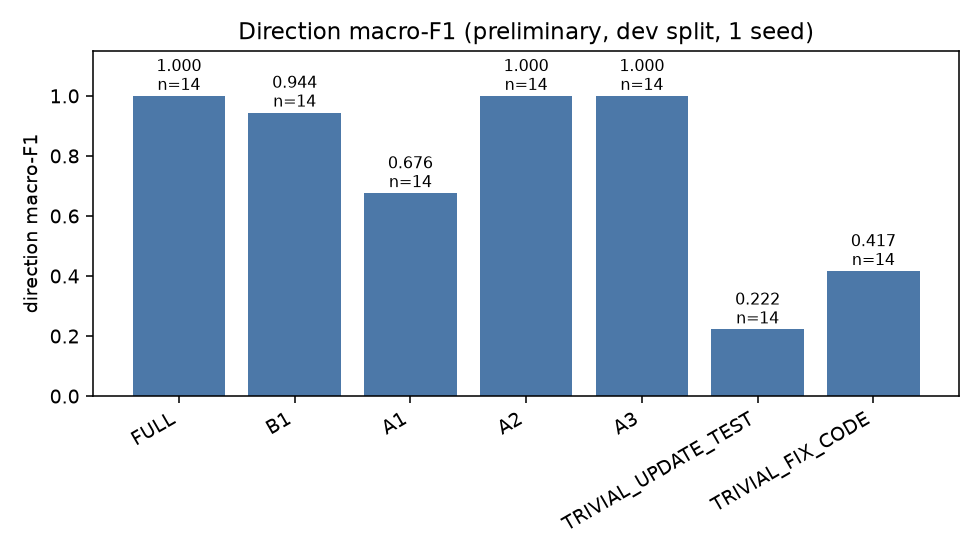
\includegraphics[width=0.60\textwidth]{figures/direction_macro_f1.png}\\{\small Direction macro-F1 on the development split}\end{center}
\begin{center}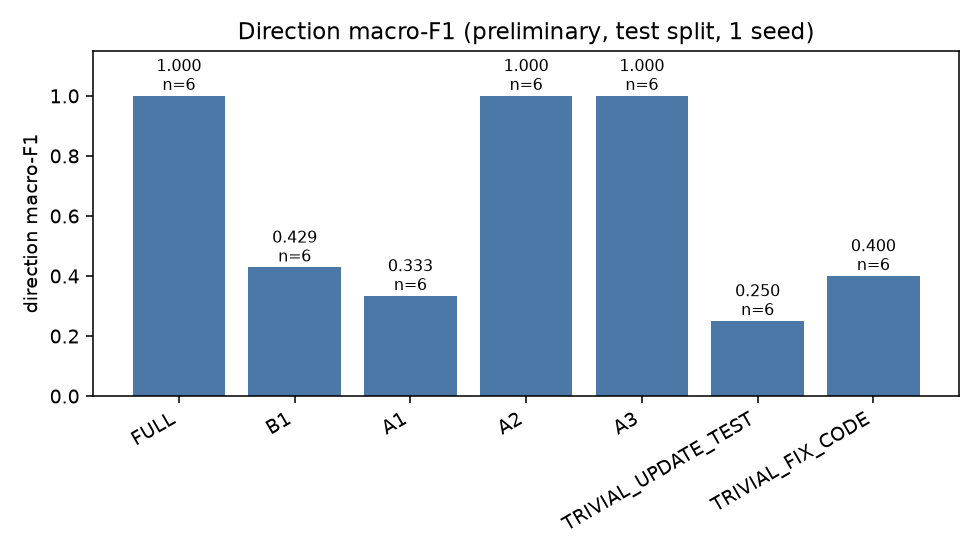
\includegraphics[width=0.60\textwidth]{figures/test_direction_macro_f1.png}\\{\small Direction macro-F1 on the frozen test split}\end{center}
\begin{center}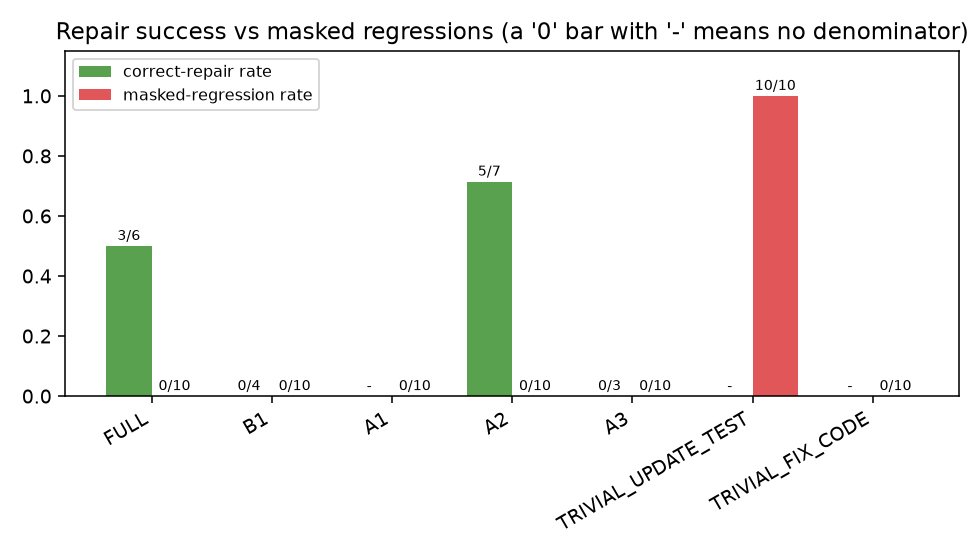
\includegraphics[width=0.60\textwidth]{figures/repair_vs_masked.png}\\{\small Repair success against masked regressions}\end{center}
\textbf{How to read the results.}

\begin{itemize}
\item Direction is scored from the agent's hypothesis, so it is generous. An escalation counts by the side it blamed. Final-action accuracy is lower because conditions escalate often; read it with direction.
\item Correct-repair rates have denominators of 1 to 7 repairs. 'Unverifiable' means a repair was accepted but no trusted probe confirmed it (A3 and B1 have no Guard).
\item Masked regressions are 0 for every model condition because none edited a test to hide a regression. The metric only separates conditions from always-UPDATE\_TEST. It does not show that the Guard is needed.
\item A1 escalated every decision, so its repair rate is undefined; its direction score comes from the hypothesis alone.
\item The post-hoc audit found no weakened and no wrong-side accepted repair in any condition. Mutant-kill retention is pooled over only the test patches whose reference tests kill a mutant (raw counts above).
\item \textbf{Limitations:} one seed, one model, 9 (+4) episodes, one library; no confidence intervals; citation support, stale-evidence rate and memory over-generalisation are not computed; Docker untested; scenario T not wired.
\end{itemize}
\textbf{One success and one failure from the logs.} dev-03 (FULL): the Analyst cited the commit message and the docstring, the source patch applied, the Guard's mutants passed, the suite was green and a memory record was written. dev-05 (FULL, A2, A3): the hypothesis was correct (outdated test) but both repair attempts edited more than expected literals and the patch-content rule refused them, so the run escalated although the direction was right. This is the strict safety rule working, and its cost.

\textbf{Reading the frozen test-split runs} (hand review of \texttt{review\_runs.py} output on \texttt{results/day4/pilot-test-5cond}; one run per cell, so these are observations, not effects).

\begin{itemize}
\item \textbf{Success, test-01 (S2, gold FIX\_CODE), FULL:} the Analyst cited the commit message, the Repairer's source patch applied, the Guard approved after the mutants were run, the suite passed and a memory record was written. A2 and A3 reached the same repair.
\item \textbf{Failure, test-02 (S2, gold FIX\_CODE), all five conditions:} every condition escalated. Each hypothesised a regression correctly but cited no expected-behaviour evidence, so the decision policy escalated. Final-action accuracy is therefore 0 on this episode for all of them, although direction was right.
\item \textbf{Failure, test-03 (S3 mixed):} for the outdated half, FULL and A2 had their test patches refused by the literal-only rule (the model changed more than expected values), while A3 and B1 produced diffs that did not apply. All escalated. For the regression half only A2 produced a Guard-approved source fix; FULL and A3 escalated for missing evidence.
\item \textbf{Decoy, test-04 (S4, gold FIX\_CODE):} FULL and A3 read the decoy memory record (its probe passed) but hypothesised a regression without citing it, and escalated. A1 cited the decoy record for an outdated-test hypothesis (the wrong direction): the only run in which a hypothesis followed the decoy, and its escalation meant no wrong-side edit was made. B1, with no memory, fixed the code correctly.
\item \textbf{B1 on test-01:} it hypothesised an outdated test for a real regression. Its two test edits were refused by the patch rule, so the masked regression was blocked by a tool rule, not by B1's judgment.
\item \textbf{What this means:} on 4 episodes the ordering by direction macro-F1 (FULL, A2, A3 above B1 and A1) is driven by a few tests: B1 is wrong on test-01 and on both test-03 rotate\_file tests, A1 on both rotate\_file tests and on test-04, and final-action accuracy is low everywhere because the evidence and patch-content rules turn most decisions into escalations. This is evidence about the policy's conservatism, not about which design is better.
\end{itemize}
\section*{7. Challenges faced and mitigation plans}
\begin{longtable}{|>{\raggedright\arraybackslash\footnotesize}p{0.387\textwidth}>{\raggedright\arraybackslash\footnotesize}p{0.473\textwidth}|}
\hline
\textbf{Challenge} & \textbf{Mitigation} \\ \hline\endhead
Free-tier quota and 503 overload (7 of 19 Day-2 runs were api\_failure) & Key pool with quota memory, retries, api\_failure never scored, --retry-failed with memory-order guard \\ \hline
Prompt contamination: Day-2 repair prompts contained dev-05 content & Fixed in repair-v5; a test fails if a prompt shares 20 characters with any pilot episode; old records kept with a notice \\ \hline
A1 side channel: commit message reachable by retrieval or read\_file & Corpus, search\_repo and non-code read\_file withheld in A1; checked by tests \\ \hline
Strict test-patch rule causes escalations (dev-05) & Report as a cost of safety; consider more allowed setup edits only on the development split \\ \hline
Mutation strength unmeasurable for small functions (dev-06: reference test kills 0 of 2 mutants) & More mutant operators and a separate 'strength unmeasurable' class in the final 15 days \\ \hline
A1 and probe-less repairs are scored ambiguously & Report direction and final-action accuracy side by side; decide the scoring rule before the final run \\ \hline
Bubblewrap only; Docker daemon not accessible & Test Docker on a machine with access, keep bwrap as the fallback \\ \hline
Small pilot cannot support statistics & Scale to three libraries and 72 episodes, two seeds, paired bootstrap \\ \hline
\end{longtable}
\section*{8. Updated repository and reproducibility}
\begin{itemize}
\item Repository: this project's \texttt{main} branch; \texttt{README.md} has the setup, \texttt{docs/interfaces.md} the interfaces and \texttt{docs/day*-*.md} the per-day logs.
\item Setup: Python 3.12 virtual environment, \texttt{pip install -e .[dev,report]}, \texttt{.env} from \texttt{.env.example} (keys are never committed), a clone of boltons at the pin and its pilot venv, bubblewrap.
\item Offline checks: \texttt{python -m pytest -q} (no API calls). Live runs: \texttt{scripts/run\_experiment.py}, then \texttt{scripts/audit\_integrity.py}, \texttt{scripts/summarize\_results.py}, \texttt{scripts/make\_report.py}.
\item Every table in this report is produced by \texttt{docs/report/build\_report.py} from \texttt{results/**/runs.jsonl}.
\end{itemize}
\section*{9. Completion plan, 31 October to 14 November}
\begin{longtable}{|>{\raggedright\arraybackslash\footnotesize}p{0.155\textwidth}>{\raggedright\arraybackslash\footnotesize}p{0.705\textwidth}|}
\hline
\textbf{Dates} & \textbf{Work} \\ \hline\endhead
Oct 31 - Nov 2 & Stabilise dataset and environments; episode-construction scripts; select the three held-out libraries; validate gold labels; pin dependencies; development stream \\ \hline
Nov 3 - 5 & Finish core features: hybrid retrieval, memory, Guard, fault recovery; fix the A1 and escalation scoring; freeze model and configuration on development data \\ \hline
Nov 6 - 9 & Full evaluation: 72-episode test set for FULL and B1 (two seeds), then A1, A2, A3 and sanity baselines, checkpointed. Throughput check first: about 74 s per run and 400k tokens for 45 pilot runs \\ \hline
Nov 10 - 11 & Metrics, paired statistics where feasible, failure analysis, test-weakening and incorrect-repair review \\ \hline
Nov 12 - 13 & Final report, plots, reproducibility package, demo \\ \hline
Nov 14 & Clean setup test, repository check, backups, final release; Nov 15 is submission only \\ \hline
\end{longtable}
\section*{10. Demo and known limitations}
Demo: \texttt{bash scripts/demo.sh} runs offline, with no API call, and writes nothing under \texttt{results/}. It rebuilds the CI state of dev-03 and shows its real failing tests, then replays the saved FULL run (evidence cited, decision, accepted patch, Guard approval), the saved B1 and A3 runs on the same episode, a no-model baseline through \texttt{scripts/run\_episode.py}, and the results table rebuilt from the saved records. The commands, expected output, an actual transcript and a terminal recording (\texttt{scriptreplay}) are in \texttt{docs/demo/}. A live run with the model is possible (\texttt{scripts/run\_episode.py --condition A2 --episode dev-03}) but spends API quota and was not used for the demo. Known limitations are listed in Sections 3 and 6.

\end{document}
